\documentclass[a4paper,14pt]{article} % тип документа
%\documentclass[14pt]{extreport}
\usepackage{extsizes} % Возможность сделать 14-й шрифт


\usepackage{geometry} % Простой способ задавать поля
\geometry{top=25mm}
\geometry{bottom=35mm}
\geometry{left=20mm}
\geometry{right=20mm}

\setcounter{section}{0}

%%%Библиотеки
%\usepackage[warn]{mathtext}
%\usepackage[T2A]{fontenc} % кодировка
\usepackage[utf8]{inputenc} % кодировка исходного текста
\usepackage[english,russian]{babel} % локализация и переносы
\usepackage{caption}
\usepackage{listings}
\usepackage{amsmath,amsfonts,amssymb,amsthm,mathtools}
\usepackage{wasysym}
\usepackage{graphicx}%Вставка картинок правильная
\usepackage{float}%"Плавающие" картинки
\usepackage{wrapfig}%Обтекание фигур (таблиц, картинок и прочего)
\usepackage{fancyhdr} %загрузим пакет
\usepackage{lscape}
\usepackage{xcolor}
%\usepackage{indentfirst}
\usepackage[normalem]{ulem}
\usepackage{hyperref}




%%% DRAGON STUFF
\usepackage{scalerel}
\usepackage{mathtools}
\DeclareMathOperator*{\myint}{\ThisStyle{\rotatebox{25}{$\SavedStyle\!\int\!\!\!$}}}
\usepackage{scalerel}
\usepackage{graphicx}
%%% END 

%%%Конец библиотек




%%%Настройка ссылок
\hypersetup
{
colorlinks=true,
linkcolor=blue,
filecolor=magenta,
urlcolor=blue
}
%%%Конец настройки ссылок


%%%Настройка колонтитулы
	\pagestyle{fancy}
	\fancyhead{}
	\fancyhead[L]{Вопрос по выбору}
	\fancyhead[R]{Талашкевич Даниил, группа Б01-009}
	\fancyfoot[C]{\thepage}
%%%конец настройки колонтитулы



\begin{document}
%%%%Начало документа%%%%


%%%Начало титульника
\begin{titlepage}

	\newpage
	\begin{center}
		\normalsize Московский физико-технический институт \\(госудраственный 			университет)
	\end{center}

	\vspace{6em}

	\begin{center}
		\Large Устный экзамен по физике (термодинамика)\\Вопрос по выбору
	\end{center}

	\vspace{1em}

	\begin{center}
		\large \textbf{Термодинамическая устойчивость}
	\end{center}

	\vspace{2em}

	\begin{center}
		\large Талашкевич Даниил\\
		Группа Б01-009
	\end{center}

	\vspace{\fill}

	\begin{center}
	Долгопрудный \\2021
	\end{center}
	
\end{titlepage}
%%%Конец Титульника



%%%Настройка оглавления и нумерации страниц
\thispagestyle{empty}
\newpage
\tableofcontents
\newpage
\setcounter{page}{1}
%%%Настройка оглавления и нумерации страниц


%%%%%%Начало работы с текстом%%%%%%

\section{Что такое термодинамическое равновесие?}
Предоставленная самой себе,
изолированная система приходит в состояние термодинамического равновесия, характеризуемое тем, что в нем все макроскопические процессы
прекращаются, скорости прямых и обратных реакций сравниваются, давление и температура принимают постоянные по объему системы значения.


Сформулированное утверждение есть обобщение опыта, и принимается
в качестве постулата — основного или общего начала термодинамики.
Состояние, близкое к термодинамически равновесному, может устанавливаться и в открытой системе. Для этого необходимо, чтобы ее энергои массообмен с окружающей средой был мал. Тогда данная система будет
вести себя почти как изолированная.
Состояние равновесия является динамическим: на молекулярном (микроскопическом) уровне непрерывно происходят сложные движения, а на
макроскопическом уровне — никаких видимых изменений.
Если параметры системы меняются от точки к точке и с течением
времени, то ее состояние — неравновесное.

\section{Условия термодинамической устойчивости}

\subsection{ Термодинамические неравенста.}

\begin{center}
	{\centering 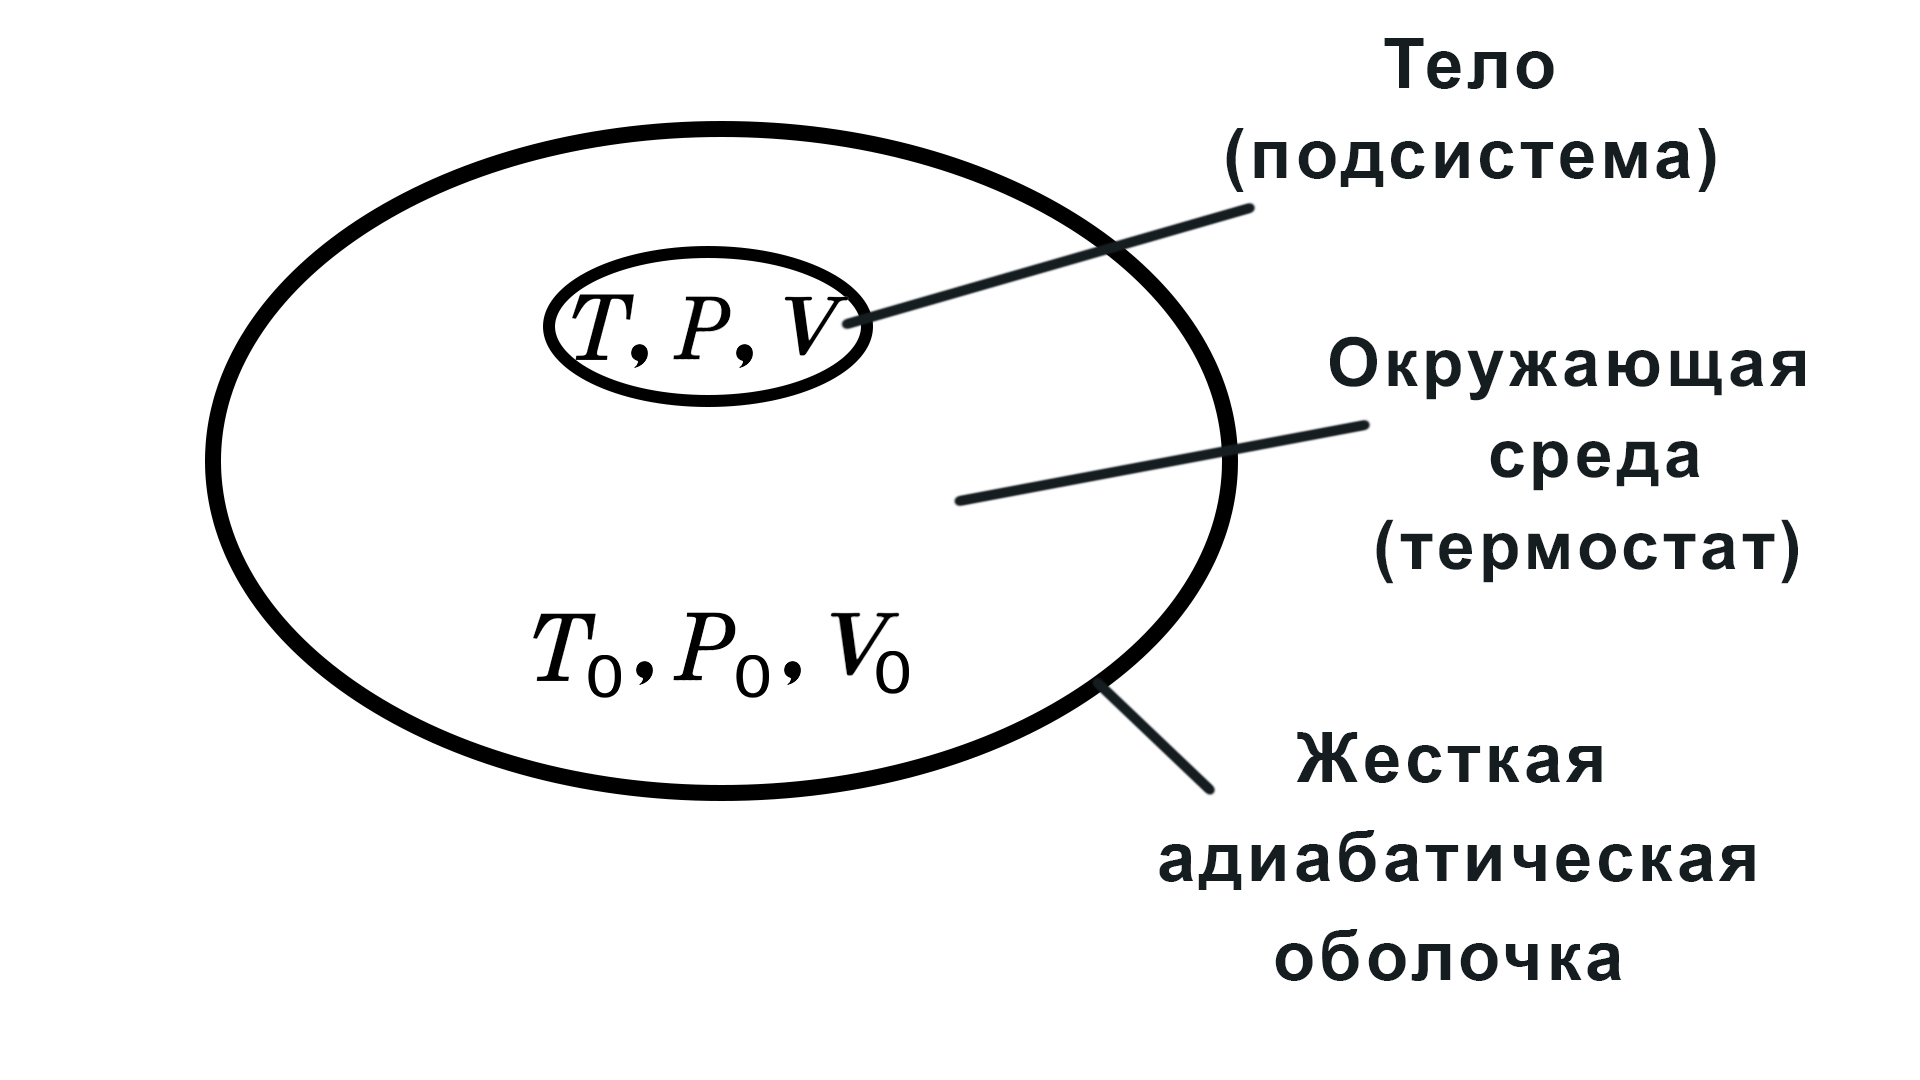
\includegraphics[scale=0.1]{PICTURE_1.jpg}}	
\end{center}

Рассмотрим систему «тело + термостат» или, иначе, «подсистема + окружающая среда», причем вся система помещена в жесткую адиабатическую оболочку. Пусть тело характеризуется параметрами $(T, P, V)$, а
термостат — $(T_0, P_0, V_0)$. Первое начало термодинамики для тела записывается в виде:

\[dU = \delta A^\swarrow  + \delta Q^\swarrow \]
где $\delta A^\swarrow$ -- работа совершенная окружающей средой над телом, а $\delta Q^\swarrow$ -- теплота, полученная телом из окружающей среды. \\
Так как оболочка жесткая, то
\[dV  = -dV_0, \delta A^ \swarrow = P_0 dV_0 = -P_0 dV\]
Согласно неравенству Клаузиуса
\[\delta Q^\swarrow \leq T_0 dS\]
где $S$ — энтропия тела, $T_0$ — температура резервуара, с которым происходит теплообмен (температура окружающей среды). С учетом
этого имеем
\[0 = dU - \delta A^\swarrow - \delta Q ^ \swarrow = dU + P_0 dV - \delta Q ^ \swarrow \geq dU + P_0dV - T_0 dS \equiv dZ\]
где введено обозначение $Z = U + P_0V - T_0 S$. Следовательно, эволюция
протекает так, что $dZ \leq 0$.\\
В состоянии равновесия величина $Z$ достигает минимума. Рассмотрим
$Z$ как функцию объема и энтропии:
\[Z = Z (V,S)\]

\subsection{Условие экстремальности Z}
\[Z: \left(\frac{\partial Z}{\partial V}\right)_S = 0, \left(\frac{\partial Z}{\partial S}\right)_V = 0\]

Имея ввиду, что для квазистатических процессов $dU = T dS - p dV$, находим

\[\left(\frac{\partial U}{\partial V}\right)_S + P_0 = -P + P_0 = 0 \Rightarrow P = P_0\]

\[\left(\frac{\partial U}{\partial S}\right)_V - T_0 = T - T_0 = 0 \Rightarrow T = T_0\]

\subsection{Условие минимума Z}
В точке экстремума $d^2Z \geq 0$ или, вследствие
постоянства $P_0$ и $T_0$, $d^2 U \geq 0$. Последнее означает

\begin{equation}
	\left(\frac{\partial^2 U}{\partial S^2}\right)_V dS^2 + 2 \left(\frac{\partial^2 U}{\partial S \partial V}\right) dS dV + \left(\frac{\partial^2 U}{\partial V^2}\right)_S dV^2 \geq 0
	\label{1.5.1}
\end{equation}


В левой части неравенства стоит квадратичная форма относительно $dS$
и $dV$. Условия ее положительной определенности есть

\[\text{а)}\left(\frac{\partial^2 U}{\partial S^2}\right)_V \textgreater 0\]

\[\text{б)} X \equiv \left(\frac{\partial^2 U}{\partial S^2}\right)_V \left(\frac{\partial^2 U}{\partial V^2}\right)_S - \left(\frac{\partial^2 U}{\partial S \partial V}\right)^2 \textgreater 0\]

Эти неравенства преобразуются с учетом соотношений

\[\left(\frac{\partial U}{\partial S}\right)_V = T, \left(\frac{\partial U}{\partial V}\right)_S = -p\]

\subsubsection{Условие а)}

\begin{equation*}
	\left(\frac{\partial^{2} U}{\partial S^{2}}\right)_{V}=\left(\frac{\partial T}{\partial S}\right)_{V}=\frac{T}{C_{V}}>0, \quad \text { т. e. } \quad C_{V}>0
\end{equation*}

\subsubsection{Условие б)}

\begin{equation}
	\begin{aligned}
		X=\left(\frac{\partial^{2} U}{\partial S^{2}}\right)_{V}\left(\frac{\partial^{2} U}{\partial V^{2}}\right)_{S} &-\left(\frac{\partial}{\partial V}\left(\frac{\partial U}{\partial S}\right)_{V}\right)\left(\frac{\partial}{\partial S}\left(\frac{\partial U}{\partial V}\right)_{S}\right)=\\
		&=-\left(\frac{\partial T}{\partial S}\right)_{V}\left(\frac{\partial P}{\partial V}\right)_{S}+\left(\frac{\partial T}{\partial V}\right)_{S}\left(\frac{\partial P}{\partial S}\right)_{V}>0 .
	\end{aligned}
	\label{1for}
\end{equation}

Рассматривая давление как функцию объема и температуры $P=P(V, T)$ имеем $d P=(\partial P / \partial V)_{T}dV + \left(\partial P / \partial T)_{V} d T\right.$, откуда

\begin{equation*}
	\left(\frac{\partial P}{\partial V}\right)_{S}=\left(\frac{\partial P}{\partial V}\right)_{T}+\left(\frac{\partial P}{\partial T}\right)_{V}\left(\frac{\partial T}{\partial V}\right)_{S}.
\end{equation*}

Подстановка последнего равенства в (\ref{1for}) дает

\begin{equation*}
	\begin{aligned}
		&X=-\left(\frac{\partial T}{\partial S}\right)_{V}\left[\left(\frac{\partial P}{\partial V}\right)_{T}+\left(\frac{\partial P}{\partial T}\right)_{V}\left(\frac{\partial T}{\partial V}\right)_{S}\right]+ \\
		&\ \ \ \ \ \ \ \quad+\left(\frac{\partial T}{\partial V}\right)_{S}\left(\frac{\partial P}{\partial S}\right)_{V}=-\left(\frac{\partial T}{\partial S}\right)_{V}\left(\frac{\partial P}{\partial V}\right)_{T}- \\
		&\ \ \ \ \ \ \ \ \ \ \ \ \ -\left(\frac{\partial T}{\partial S}\right)_{V}\left(\frac{\partial P}{\partial T}\right)_{V}\left(\frac{\partial T}{\partial V}\right)_{S}+\left(\frac{\partial T}{\partial V}\right)_{S}\left(\frac{\partial P}{\partial S}\right)_{V} .
	\end{aligned}
\end{equation*}

Имея в виду, что
$$
\left(\frac{\partial T}{\partial S}\right)_{V}=\frac{T}{C_{V}}, \quad\left(\frac{\partial T}{\partial S}\right)_{V}\left(\frac{\partial P}{\partial T}\right)_{V}=\left(\frac{\partial P}{\partial S}\right)_{V},
$$
получим
$$
X=-\frac{T}{C_{V}}\left(\frac{\partial P}{\partial V}\right)_{T}>0 .
$$
Вследствие неравенства $C_{V}>0$ получаем, что $(\partial P / \partial V)_{T}<0 .$ Таким образом, независимо от уравнения состояния вещества изотермическая сжимаемость

\begin{equation*}
	\beta_{T}=-\frac{1}{V}\left(\frac{\partial V}{\partial P}\right)_{T}>0.
\end{equation*}

Поскольку 

\begin{equation*}
	C_{P}-C_{V}=-T \frac{(\frac{\partial V} {\partial T})_{P}^{2}}{(\frac{\partial V}{ \partial P})_{T}},
\end{equation*}

то из полученного неравенства следует, что всегда $C_{P}>C_{V} .$ Имея в виду также, что $C_{V}>0$, заключаем, что показатель адиабаты $\gamma=C_{P} / C_{V}>1 .$ Для положительной определенности квадратичной формы в (\ref{1.5.1}) можно было бы условие \textbf{а)} заменить условием $\left(\partial^{2} U / \partial V^{2}\right)_{S}>0$ или $\left(\partial^{2} U / \partial V^{2}\right)_{S}=-(\partial P / \partial V)_{S}>0 .$ Последнее означает, что адиабатическая сжимаемость также положительна:

\begin{equation*}
	\beta_{T}=-\frac{1}{V}\left(\frac{\partial V}{\partial P}\right)_{T}>0.
\end{equation*}

Условия термодинамической устойчивости $C_V > 0$ и $\beta_{T} > 0$ называют 
термодинамическими неравенствами.

\section{Смысл условий устойчивости}

Предположим, что подсистема находится в тепловом и механическом равновесии с внешней средой, т. е. $T=T_{0},\ P=P_{0} .$ Покажем, что при нарушении найденных условий состояние равновесия не может быть устойчивым.

1) Допустим, что $C_{V}<0 .$ Пусть температура подсистемы случайно уменышилась, $T<T_{0} .$ Тогда в соответствии со вторым началом термодинамики в эту подсистему потечет тепловой поток из внешней среды. Поскольку $\delta Q=C_{V} d T>0$, то в результате температура $T$ еще более уменьшится. Аналогично, случайное увеличение температуры подсистемы приведет к ее дальнейшему увеличению. Следовательно, тепловое равновесие неустойчиво.

2) Допустим, что $(\partial \boldsymbol{P} / \partial \boldsymbol{V})_{\boldsymbol{T}}>\mathbf{0 .}$ Пусть объем подсистемы случайно уменьшился. Тогда давление в ней также уменьшилось, $P<P_{0} .$ В результате внешнее давление $P_{0}$ оказывается больше, чем внутреннее. Поэтому объем подсистемы будет и дальше уменьшаться. Аналогично, при случайном увеличении объема подсистемы ее объем будет продолжать увеличиваться. Следовательно, механическое равновесие оказывается неустойчивым.

\section{Общие критерии термодинамической устойчивости}

\subsection{Критерий термодинамической устойчивости.}

Допустим, что адиабатически изолированная система находится
в термодинамическом равновесии, причем ее энтропия $S$ в рассматриваемом состоянии максимальна, т. е. больше энтропии всех возможных бесконечно близких состояний, в которые система может перейти без подвода или отвода тепла. \\

Тогда можно утверждать, что
самопроизвольный адиабатический переход системы во все эти состояния невозможен, т. е. система находится в устойчивом термодинамическом равновесии.\\

Действительно, если бы такой переход
был возможен, то энтропии начального 1 и конечного 2 состояний
были бы связаны соотношением $S_1 > S_2$. Но это соотношение находится в противоречии с принципом возрастания энтропии, согласно
которому при адиабатических переходах должно быть $S_1 < S_2$.
Таким образом, мы приходим к следующему критерию термодинамической устойчивости.\\

\textit{Если система адиабатически изолирована и ее энтропия в некотором равновесном состоянии максимальна, то это состояние
является термодинамически устойчивым. Это значит, что система,
оставаясь адиабатически изолированной, не может самопроизвольно
перейти ни и как;е другие состояние.}\\

В приложениях термодинамики к конкретным вопросам часто
бывает удобно вместо адиабатической изоляции системы накладывать
на ее поведение другие ограничения. Тогда критерии термодинамической устойчивости изменятся. Особенно удобны два достаточных условия. 

\subsection{Первое достаточное условие}

Пусть система окружена средой, температура которой поддерживается постоянной. Кроме того, объем системы $V$ также поддерживается постоянный, например, система заключена в жесткую оболочку. В этих условиях работа системы $A$ всегда равна нулю, и соотношение

\begin{equation*}
A\leqslant Y_{1}-Y_{2},
\end{equation*}

где $Y = U - T_0S$, а само соотношение -- следствие из неравенства Клаузиуса, переходит в $Y_{1}-Y_{2} \geqslant 0 .$ Следовательно, функция $Y \equiv U-T_{0}$. может только уменьшаться или оставаться неизменной. Отсюда, рассуждая, как и раньше, получаем следующий критерий термодинамической устойчивости.

\textit{Если температира окружающей среды $T_{0}$ и объем системы $V$ поддерживают постоянными и в рассматриваемом состоянии функция $Y=U-T_{0}S$ минимальна, то состояние системы термодинамически устойчиво. В частности, если температура среды равна температуре системы, роль функции $Y$ выполняет свободная энергия $\Psi=U - T S$.}

\subsection{Второе достаточное условие}

Допустим теперь, что система со всех сторон окружена средой, температура $T_{0}$ и давленне $P_{0}$ которой поддерживаются постоянными. Никакой работы, помимо работы против внешнего давления $P_{0}$ система совершать не может. Иными словами, полезная работа системы всегда равна нулю, так что соотношение 

\begin{equation*}
A^{\text {полезное}} \leqslant Z_{1}-Z_{2},
\end{equation*}

где 

\begin{equation*}
Z=Y+P_{0} V=U-T_{0} S+P_{0} V,
\end{equation*}

 дает $Z_{2} \leqslant Z_{1} .$ Все самопроизвольные процессы в системе могут идти только с уменьшением функции $Z \equiv Y+P_{0} V .$ Поэтому, \textit{если финкция $Z$ В некотором равновесном состоянии достигла минимума, то равновесие будет устойчивым. В частности, когда $P = P_0$,  это утверждение относится к термодинамическому потенциалу системы $\Phi = F+ P V$.}
 
Приведем еще два, менее употребительные, условия термодинамической устойчивости. В них роль потенциалыных функций выполняют внутренняя энергия $U$ и энтальпия $I$.

\subsection{Менее полезные условия термодинамической устойчивости}

\textbf{1}. Перепишем неравенство Клаузиуса в виде
\[S_2 - S_1 \geq \myint_{1\rightarrow 2}{\frac{dU + \delta A}{T}}\]
Пусть энтропия и объем системы поддерживаются постоянными. Тогда $S_2 - S_1 = 0$ и $\delta A = PdV = 0$, поэтому предыдущее неравенство дает 
\[\myint{\frac{dU}{T}} \leq 0\]
Так как $T > 0$, то отсюда следует, что $dU \leq 0$. Если объем и
энтропию системы поддерживать постоянными, то самопроизвольные процессы в ней могут идти лишь с уменьшением внутренней
энергии. Если внутренняя энергия системы достигла минимума, то
дальнейшие процессы в системе становятся невозможными. Это
приводит к следующему критерию термодинамической устойчивости.\\\\
\textit{Если объем и энтропия системы поддерживаются постоянными
и система в некотором равновесном состоянии достигла минимума
внутренней энергии, то равновесие термодинамически устойчиво.} 

\textbf{2}. Если давление и энтропия системы поддерживаются постоянными и система, в некотором равновесном состоянии достигла минимума энтальпии, то равновесие термодинамически устойчиво.
Для доказательства этого положения следует переписать неравенство Клаузиуса в виде 
\[S_2 - S_1 \geq \myint_{1\rightarrow 2}{\frac{dU - VdP}{T}}\]
и повторить предыдущие рассуждения.

\section{Неравенство Клаузиуса}
При выводе некоторых формул мы использовали неравенство Клаузиуса, поэтому, на последок, сформулируем и докажем его.

\begin{center}
	{\centering 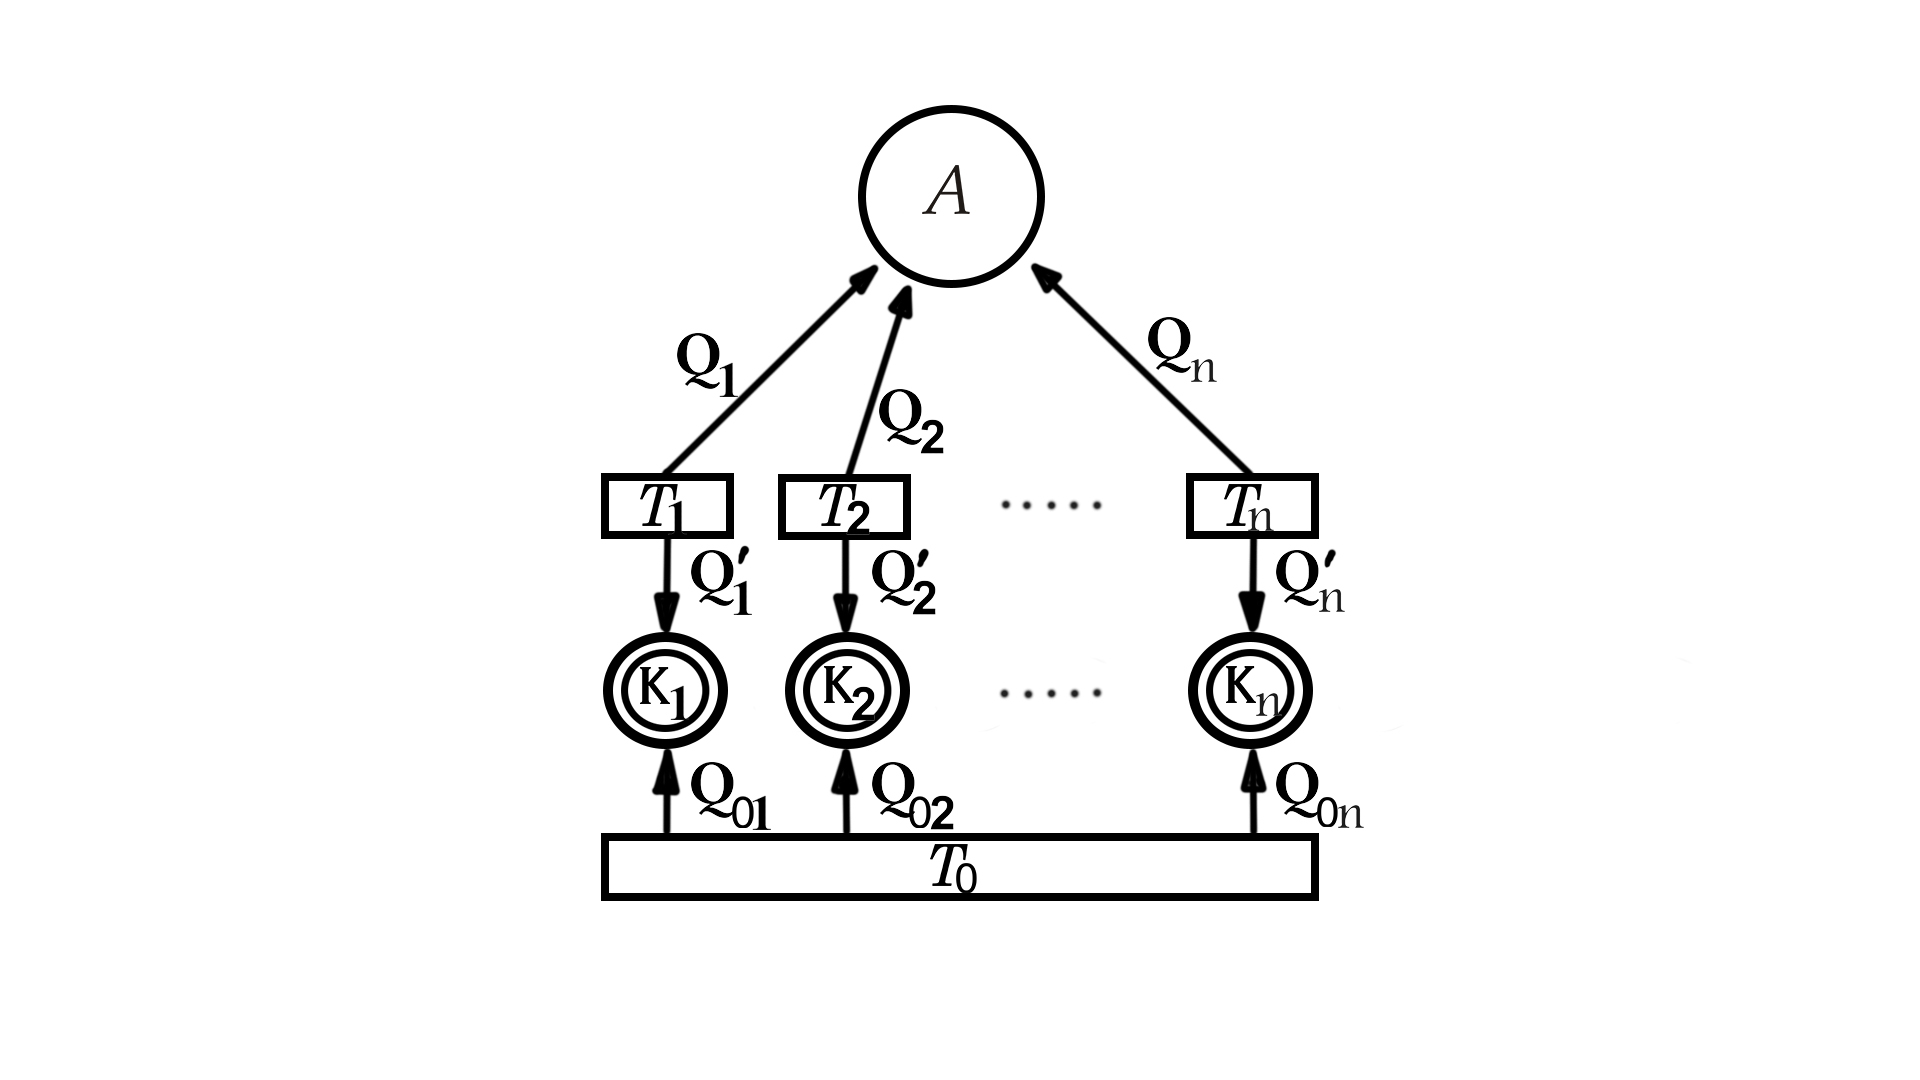
\includegraphics[scale=0.2]{PICTURE_2.jpg}}	
\end{center}

Согласно второй теореме Карно $\eta \leq \eta_k$, где $\eta_k$ — КПД машины Карно. Отсюда следует, что $1 - \frac{Q_2^\nearrow}{Q_1^\swarrow} \leq 1 - \frac{T_2}{T_1}$. Поскольку $Q_2^\nearrow = - Q_2^\swarrow$, а $Q_1^\swarrow > 0$ (По определению КПД), то мы приходим к частному случаю неравенства Клаузиуса:
\[\frac{Q_1^\swarrow}{T_1} + \frac{Q_2^\swarrow}{T_2} \leq 0\]
Для обратимой машины, работающей
только с двумя резервуарами, справедливо равенство Клаузиуса:
\[\frac{Q_1^\swarrow}{T_1} + \frac{Q_2^\swarrow}{T_2} = 0\]

Пусть теперь система А осуществляет произвольный круговой процесс. Рассмотрим ее контакт с набором $п$ термостатов, имеющих температуры $T_i$. Для восстановления состояния резервуаров введем вспомогательный резервуар с температурой $T_0$ и $n$ машин Карно, осуществляющих перекачку тепла из резервуара $T_0$ в резервуар $T_i$. Для каждой машины Карно согласно равенству Клаузиуса имеем
\[\frac{Q_{0i}}{T_0} + \frac{Q_i'}{T_i} = 0\]
или
\[Q_0 = \sum\limits_{i = 1}^n Q_{0i} = -T_0\sum\limits_{i=1}^n \frac {Q_i'}{T_i}\]
(стрелку [$^{\swarrow}$] не пишем для краткости). Подберем теплоты $Q_{i}^{\prime}$ так, чтобы они полностью компенсировали расходы резервуаров $T_{i}: Q_{i}^{\prime}=-Q_{i} .$ Тогда $Q_{0}=T_{0} \sum_{i=1}^{n} Q_{i} / T_{i} .$ Это количество тепла отдаст резервуар $T_{0} .$ B peзультате система $A$ совместно с машинами Карно $\mathrm{K}_{i}$ совершнт круговой процесс, фактически обмениваясь теплом с единственным резервуаром $T_{0}$. Поскольку этот резервуар отдал тепло $Q_{0}$, то совершена эквивалентная работа $A=Q_{0} .$ Согласно второму началу термодинамики в формулировке Томсона эта работа не может быть положительной: $A \leqslant 0 .$ Отсюда следует неравенство Клаузиуса (общий случай):

\begin{equation*}
\sum_{i=1}^{n} \frac{Q_{i}^{\swarrow}}{T_{i}} \leqslant 0.
\end{equation*}

Переходя к пределу бесконечно большого числа промежуточных резервуаров, обменивающихся бесконечно малыми порциями тепла с системой $A$ и резервуаром $T_0$, приходим к неравенству Клаузиуса в интегральной форме:

\begin{equation*}
\oint \frac{\delta Q^{\swarrow}}{T} \leqslant 0
\end{equation*}

Здесь величина $T$ есть температура термостата, с которым в данный
момент система обменивается теплом.

Пусть в системе $A$ протекают только обратимые процессы. Тогда процесс можно провести в обратном направлении через те же промежуточные состояния, что и прямой, изменив лишь знак поступающей в систему теплоты и совершаемой работы. Применяя неравенство Клаузиуса
для этого случая $\oint \frac{\delta Q^{\swarrow}}{T} \leqslant 0$ с учетом замены $\delta^{\prime} Q^{\swarrow}= - \delta Q^{\swarrow}$ , находим $\oint \frac{\delta Q^{\swarrow}}{T} \geqslant 0$. Совместно с неравенством Клаузиуса в исходной форме это
дает равенство Клаузиуса:

\begin{equation*}
\oint \frac{\delta Q^{\swarrow}}{T}=0
\end{equation*}

\section{Литература}

\begin{enumerate}
\item Сивухин Д. В. Общий курс физики. — М.: Наука, 1975. — Т. II. Термодинамика и молекулярная физика.

\item Ландау Л. Д., Лифшиц Е. М. Статистическая физика. Часть 1. — («Теоретическая физика», том V).

\item Кириченко Н. А. 1.3.8. Неравенство Клаузиуса // Термодинамика, статистическая и молекулярная физика. — 3-е изд. — М.: Физматкнига, 2005.
\end{enumerate}

\end{document}
